% !TEX program = xelatex

\documentclass[12pt, a4paper]{article}

\usepackage{fontspec}
\setmainfont[Ligatures=TeX]{Linux Libertine O}

\usepackage[rgb]{xcolor}
\definecolor{lightblue}{rgb}{0.4, 0.6, 0.9}
\usepackage[hidelinks, colorlinks=true, linkcolor=lightblue, urlcolor=lightblue, citecolor=lightblue, filecolor=lightblue]{hyperref}

\usepackage{indentfirst}
\usepackage{graphicx}
\usepackage[left=1.5cm,right=1.5cm,top=1.5cm,bottom=1.5cm]{geometry}
\usepackage{lipsum}
\usepackage{caption}
\usepackage{subcaption}
\usepackage{dirtytalk}
\usepackage{cancel}
\usepackage{amsmath}

\usepackage{minted}


\usepackage{nameref}
\newcommand*{\fullref}[1]{\hyperref[{#1}]{\ref*{#1} \nameref*{#1}}} 

\setlength{\parskip}{0.8em}

\usepackage{epigraph}


\graphicspath{{assets/}}


\begin{document}



\title{
Neural network training workflow in Ilastik\\[1cm]

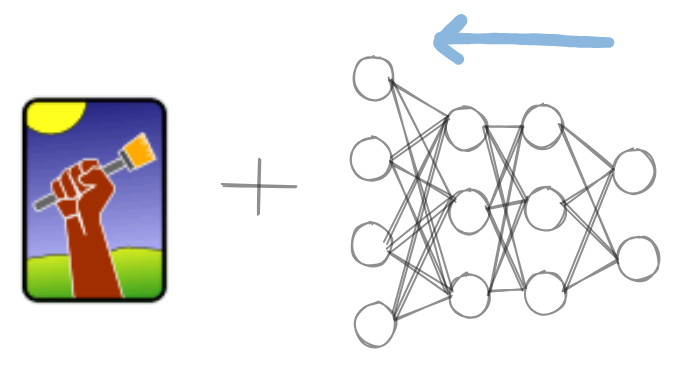
\includegraphics[width=0.5\textwidth]{ilastik-logo.png}
}

\author{Theodoros Katzalis}


\date{10/2024}

% \date{\today}

\sloppy
\maketitle

{
%\renewcommand*\contentsname{Περιεχόμενα}
\hypersetup{linkcolor=black}
\tableofcontents
}

\clearpage

\section{Introduction}

Ilastik is a desktop application that bridges the gap between machine learning and out of the box functionality intended for the bioimaging domain. For more about ilastik, check the documentation at \url{https://ilastik.github.io/}.

The main takeaway of the currently supported functionality is that training is only possible with shallow models (e.g. random forests), and neural network workflows are used only for inference. Our endeavor would be to integrate neural network training in ilastik.

The main motivation of this work originates by the shallow to deep project \cite{Matskevych2021.11.09.467925}. Its core idea is that domain adaptation can achieve greater performance by incorporating a shallow model as a preliminary step. Instead of trying to learn the mapping of raw data to the ground truth segmentations, we can learn the mapping of the output of the shallow model to the ground truth segmentations (enhancer). For a new dataset, the pretrained enhancer attempts to correct the result of the new trained shallow model. A subsequent part would be as well to train a new neural network model (segmentor) for semantic segmentation from raw images, but this time to use the output of the pretrained enhancer as pseudo labels. The whole workflow can be illustrated in the following figure:

\begin{figure}[h!]
    \centering
    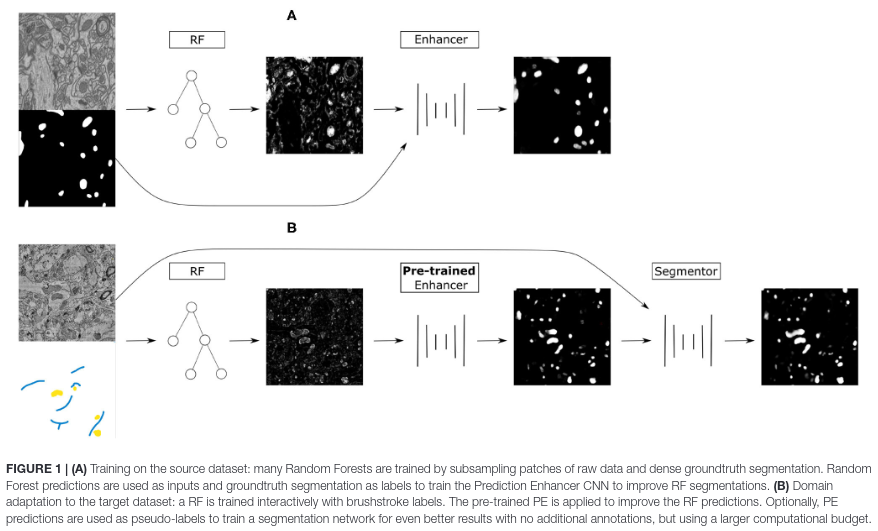
\includegraphics[width=0.8\textwidth]{shallow2deep.png}
    \caption{Shallow to deep \cite{Matskevych2021.11.09.467925}}
\end{figure}

Having as a reference point the above workflow, ilastik provides the functionality for training the random forests, but not the enhancer and the segmentor. Our goal is to achieve the whole workflow with ilastik.

Effectively to realize the above, we will attempt to implement a supervised machine learning workflow in ilastik. This will serve as the starting point for more sophisticated training workflows in the future. For next steps, refer to \fullref{sec:next_steps}.

\clearpage

\section{Ecosystem}

\begin{figure}[h!]
    \centering
    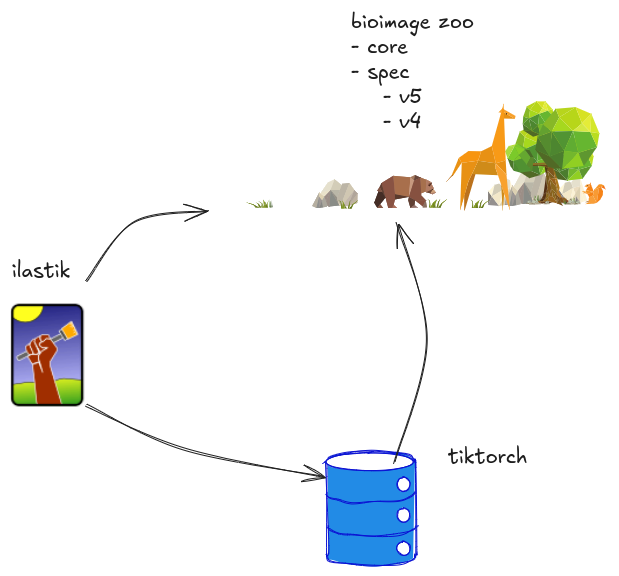
\includegraphics[width=0.8\textwidth]{ecosystem.png}
    \caption{Ecosystem}
\end{figure}

The BioImage Model Zoo provides the infrastructure to define, store, and retrieve deep learning models for the bioimage community. Currently, there are two fundamental packages, the spec-bioimage-io (\url{https://github.com/bioimage-io/spec-bioimage-io}), and the core-bioimage-io-python (\url{https://github.com/bioimage-io/core-bioimage-io-python}). In a nutshell, the first one defines a specification that describes a deep learning model (e.g. type of inputs, outputs, weights, documentation), and provides the functionality of loading and saving it. The second one is mainly responsible to run a model (e.g. inference with tiling).

Tiktorch (\url{https://github.com/ilastik/tiktorch}) attempts to manage the heavy load and orchestration of running deep learning models. The idea is that the last one is a computationally expensive task, so it could be decoupled from the client to a more suitable infrastracture (remote server). Effectively, it leverages BioImage Model Zoo to do the inference and loading of the models. Tiktorch is our backend system, and Ilastik the client.

Ilastik handles all the workflows related with shallow models. For the deep learning ones, it sends requests to Tiktorch to run the models and fetch the predictions. To avoid unnecessary communication delays for invalid requests, Ilastik does some initial validation using the BioImage Model Zoo. Regarding validation of requests refer to \fullref{sec:validation}.



\section{Current state of tiktorch}

As we have seen Tiktorch is our backend system to run the heavy load of neural networks. It supports inference of neural networks using the  BioImage Model Zoo. Let's see what is the current state of it.

producer-consumer

threads, processes, orchestration

\section{Supervised training in Ilastik}

The requirements are:

P0 - Must have
\begin{itemize}
    \item \textbf{P0.0} Ilastik must support 2d and 3d deep learning training for the semantic segmentation task.
    \item \textbf{P0.1} Training must be possible locally or remotely with GPU support.
    \item \textbf{P0.2} Ilastik must be able to render the progress of training. Rendering of the progress can be asynchronous.
    \item \textbf{P0.3} Ilastik must be able to resume, pause, and cancel a training process.
    \item \textbf{P0.4} Ilastik must be able to provide optional configuration of the model.
    \item \textbf{P0.5} Ilastik must be able to expose different model architectures (e.g. U-Net variations, ResNet).
\end{itemize}


\section{Deep learning models to use}
\label{sec:deep_models}

To satisfy \textbf{P0.0}, and \textbf{P0.5}, U-Net architecture \cite{ronnebergerUNetConvolutionalNetworks2015} will serve as the foundational one for semantic segmentation, while exposing variations such as U-Net-ResNet18, U-Net-Resnet50, etc. The 3d dataset requirement can be satisfied by using the 3d equivalent component for the 2d ones. The selection will be filtered initially by the type of the dataset, e.g. 3 dimensions (x,y,channel) for 2d datasets  and 4 dimensions (x,y,z,channel) for 3d datasets \footnote{2d and 3d images are usually refered to the spatial axes, that's why a 3d image is actually 4d, and 2d is 3d.}. What about time? 

Regarding the U-Net variations, using ResNet as backbone comes with a computational cost. Thus, we could expose U-Net implementations with a fixed number of plain convolutional and pooling layers. Potentially we could expose to configure a custom U-Net with an arbitrary number of layers. Another direction would be to leverage foundational models such as the Segment Anything For Microscopy with fine-tuning.

In theory, the list of the available models to choose could be updated over the course of the project and the design should be flexible enough to accommodate this.

We assume a fair amount of understanding from the user to estimate the complexity of the model for the target dataset. We can use as default a moderate complexity model (e.g. U-Net-ResNet-50).

What about plant-seg?


\subsection{ResNet}

The number of layers is based on \cite{heDeepResidualLearning2015}.

\begin{enumerate}
    \item U-Net-ResNet-18
    \item U-Net-Resnet-34
    \item U-Net-ResNet-50
    \item U-Net-ResNet-101
\end{enumerate}

These could have the option of being pretrained or not to ImageNet for the 2d datasets. What about kernel inflation to leverage pretrained models for the 2d images?

\subsection{Plain}

Plain U-Net configurations could be:
\begin{enumerate}
    \item U-Net with 4 convolutional layers and 1 pooling
    \item ?
\end{enumerate}


\subsection{Summary}

Make a table of the proposed models.

\subsection{Framework}

All the models will be implemented in PyTorch. What about integration with other existing implementations in Tensorflow? Should we take ths into account as well?

\section{Dataset size and tiling training}
\label{sec:tiling}

As we have mentioned, our task would be semantic segmentation, and we could provide some generic model architectures \fullref{sec:deep_models}. Another challenge would be to handle an arbitrary dataset size.

Memory constraints may not allow for a model to be trained on full images. Thus tiling based training needs to be supported. To determine if training should be based on tiles, we need to take into account the most crucial memory factors which are batch size, image shape (2d or 3d), and model's complexity (e.g. number of feature maps).

For the option of tiling based training, we need to configure the halo, and the patch size. These should be exposed to the user with sensible defaults.

Should we do inference on a patch that it is different than the one in the training?

Currently, Ilastik has some hard-coded values for the patch size for 3d and 2d images. This is just a heuristic, and we aim to improve this. The same problem applies for the training as well.

\subsection{Memory constraints}

Memory constraints are referred to the GPU usage. We assume that for neural network training a GPU is required. Thus we should possibly monitor the most impactful parameters that determine the memory usage.

Make a flowchart. What would be our memory parameter to decide about if my model fit to memory?

\section{Hyperparameter turning}

Each of the models mentioned \fullref{sec:deep_models}, they could have their own set of parameters to tune \footnote{U-Net-ResNet variations will have the same type of parameters such as batch size, learning rate optimizer, but if we support models such as custom U-Net, a new set of parameters needs to be configured such as the number of layers, number of pooling layers etc.}. Hyperparameter tuning is a heavy computational task. We could have some fixed values, and \textbf{optionally} allowing for tuning them given a user defined range of parameters.

One challenge is what kind of parameters should be tuned, and what type of hyperparameter strategy should we follow (e.g. grid search, bayesian optimization, random search).

A list of hyperparameters could include:
\begin{itemize}
    \itemsep -0.2em
    \item Epochs
    \item Batch size
    \item Optimizer (e.g. Adam, SGD)
    \item Learning rate
    \item Batch normalization
    \item Dropout layers
    \item Type of padding
    \item Loss function
    \item Kernel size, stride
    \item Patch size (\fullref{sec:tiling})
\end{itemize}



\section{Preprocessing}

What about preprocessing and normalization? Downscaling? Augmentations?


\section{Logging}

To monitor the progress of the training, we need a logging framework. There are two well knowing frameworks used in the community, 1) the weights \& biases and 2) tensorboard.


As we have seen, we will rely on existing machine learning logging frameworks. More specifically, we will assume that the logs are saved on the disk and Ilastik is able to read from that.


\section{Architecture}

High level diagram of what user will do. Provides input data, and ground truth.

\section{Remote server requirements}

As we have seen we need to be able to save logs and the checkpoints. So apart from GPU resources needed for training, we need to have write access to the disk of the remote server. Alternatively, if this isn't possible, then the logs and the checkpoints should be streamed over grpc.

\section{Tiktorch}

Orchestration of resources for training. A gpu should be used for one model training. Is it possible to train two models with the same gpu? It is a good practise to do so?

\subsection{API}

\begin{itemize}
    \item Start training
    \item Pause training
    \item Resume training
    \item Abort training
    \item Clean
\end{itemize}

\subsubsection{Start}

The start training should be responsible to initialize the model with the training parameters. This can include if hyperparameter tuning should be included or not.

\subsubsection{Pause}

Save training progress. Should each resume operation to update the last one? Or save to a separate file? Where the weights should be saved?

\subsubsection{Resume}

Load saved training progress, and continue training. 

\subsubsection{Abort}

Abort the training process, release resources and remove any logs.

\subsubsection{Clean}

This call should be responsible to remove any artifacts (e.g. logs) created during training.

\section{Lazyflow}

What kind of operators to use.

\section{Ilastik view}

How it would look like?

\section{Validation ownership}
\label{sec:validation}

Validation of requests is crucial especially over networks that introduce significant latency. For example attempting to request to run a model, realizing that it doesn't exist in the server side, is a relative slow feedback loop. It can happen from the client side to speedup the process.

For the use cases of requests from ilastik to tiktorch, currently both of them perform some validation checks. On the other hand, bioimage model zoo performs some of them as well. In more detail:

\begin{itemize}
    \itemsep -0.2em
    \item item1
    \item item2
\end{itemize}


It would probably be wise to standardize and modularize the validation. Each component should be able to perform validation, but the logic could be encapsulated in a central location. Bioimage model zoo should probably be the best candidate for that. 

\section{Next steps}
\label{sec:next_steps}

One of the major bottlenecks with supervised machine learning, and especially in the biological domain, is the very expensive and time-consuming process of data annotation. Thus unsupervised learning and transfer learning are great candidates for our use case. Some next ideas could include:

\begin{enumerate}
    \item Ilastik should be able to detach from a training process and reattach.
    \item The user should be able to provide their own model definition written in PyTorch or Tensorflow.
    \item BioImage Model Zoo integration.
    \item Representation learning. Instead of trying to train from scratch a neural network in a supervised manner, would be very beneficial to make use of the latent space of representation learning methods.
    \item Integrate already trained models (e.g. bioimage zoo), allowing finetuning to them.
    \item Instance segmentation.
\end{enumerate}

\clearpage

\bibliographystyle{plain}
\bibliography{bib.bib}



\end{document}